\documentclass[11pt]{article}

\usepackage[margin=1.5cm]{geometry}
\usepackage{amssymb}
\usepackage{booktabs}
\usepackage{graphicx}
\usepackage{longtable}
\usepackage{pdflscape}

\setlength{\LTleft}{0pt}
\setlength{\LTright}{0pt}
\renewcommand{\arraystretch}{0.98}
\providecommand{\botrule}{\bottomrule}

\title{Online Resource 1: Exploratory and Supportive Material for IVF/SPEA2}
\author{}
\date{}

\begin{document}

\maketitle

This online resource collects the exploratory average-rank figure, representative engineering-front plots, and supportive ablation material referenced in the manuscript. The per-instance synthetic IGD and HV tables are now reported in Appendix~A of the main manuscript. All supplementary items follow the same cohort definitions, filtering rules, and sign conventions described in the paper.

\clearpage
\begin{figure}[p]
	\centering
	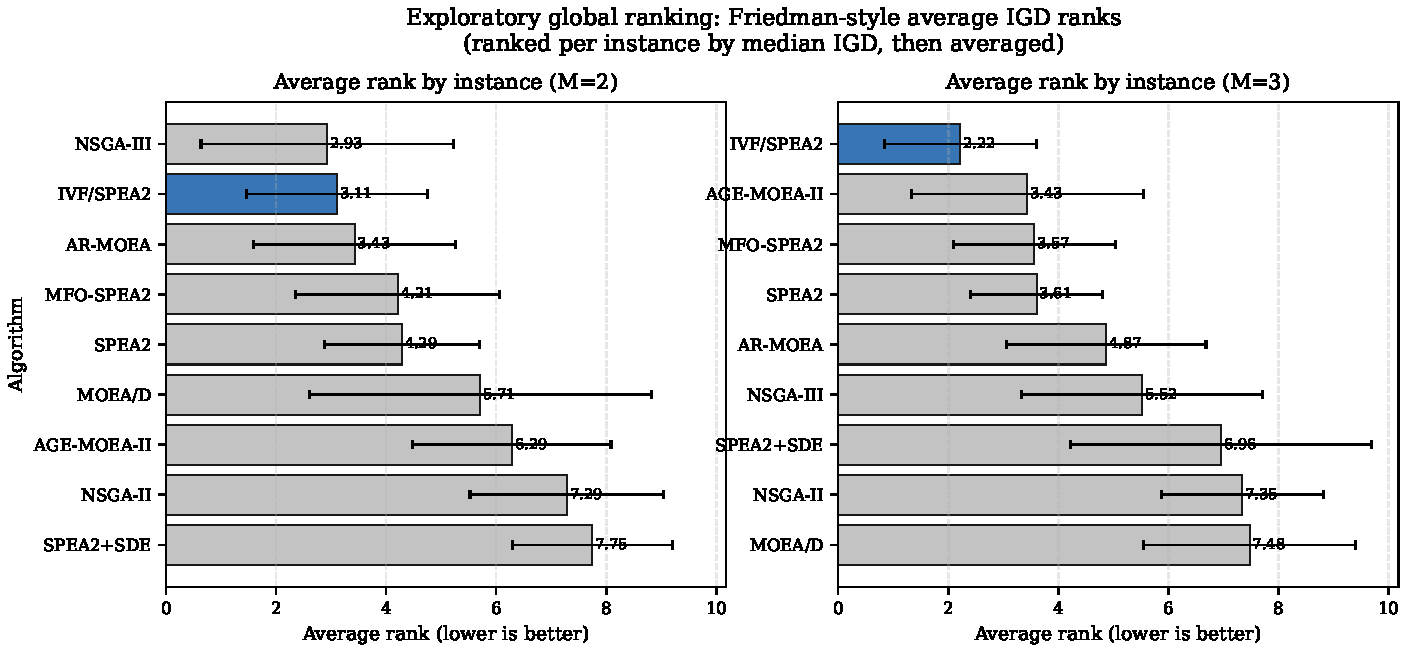
\includegraphics[width=0.92\textwidth]{../figures/friedman_avg_rank_igd.pdf}
	\caption{Exploratory Friedman-style average ranks based on per-instance median IGD. These ranks provide contextual navigation only and are not used for confirmatory claims in the main manuscript.}
\end{figure}

\clearpage
\begin{figure}[p]
	\centering
	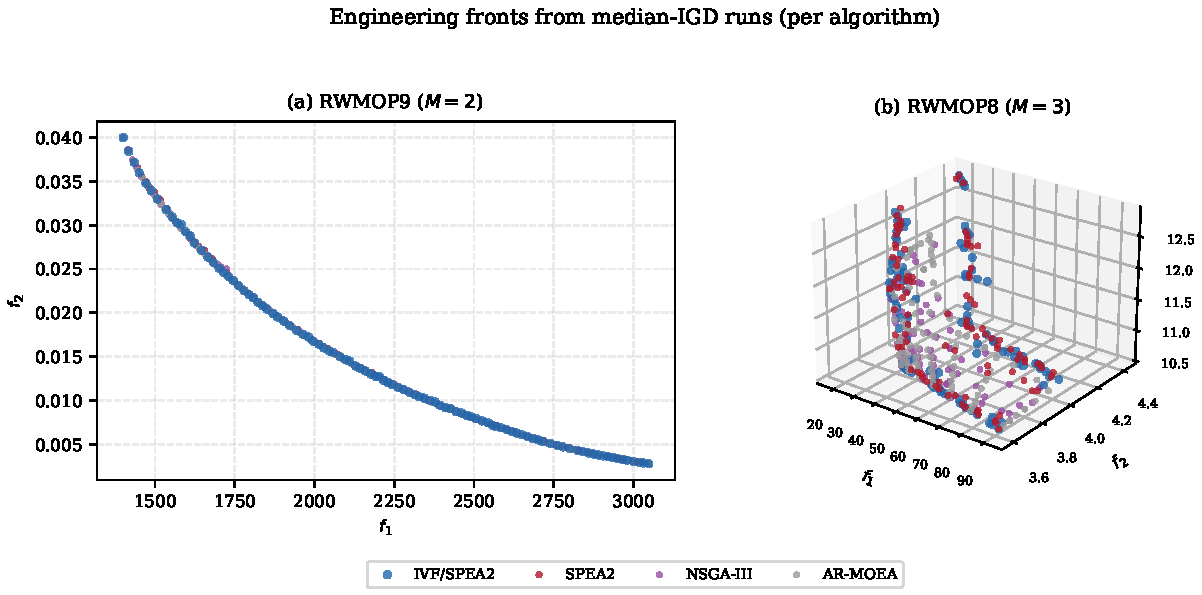
\includegraphics[width=0.86\textwidth]{../figures/engineering_fronts_rwmop9_rwmop8.pdf}
	\caption{Representative engineering fronts from the median-IGD run of each algorithm. Panel (a) shows the largely overlapping support on RWMOP9 ($M=2$), whereas panel (b) highlights the narrower low-$f_2$ concentration of NSGA-III and AR-MOEA relative to IVF/SPEA2 and SPEA2 on RWMOP8 ($M=3$).}
\end{figure}

\clearpage
{\scriptsize
	\begin{table*}[t]
\caption{Phase 1 Screening: median IGD (IQR) over 30 runs. Symbols: $+$ = variant significantly better than baseline, $-$ = significantly worse, $\approx$ = no significant difference (Wilcoxon, $\alpha=0.05$). Best median per instance in \textbf{bold}.}
\label{tab:ablation_v2_phase1}
\centering\scriptsize
\resizebox{\textwidth}{!}{%
\begin{tabular}{lrrrrrr}
\toprule
Instance & B (v1 baseline) & V1 (dissim.) & V2 (collective) & V3 ($\eta_c=10$) & V4 (adaptive) & V5 (mutation) \\
\midrule
ZDT1(M=2) & 4.03(5.00)e-2 & 3.92(0.07)e-3$^{+}$ & 3.91(0.07)e-3$^{+}$ & 3.93(0.10)e-3$^{+}$ & \textbf{3.90(0.05)e-3}$^{+}$ & 3.94(0.07)e-3$^{+}$ \\
ZDT6(M=2) & 3.07(0.03)e-3 & \textbf{3.06(0.03)e-3}$^{\approx}$ & 3.08(0.03)e-3$^{\approx}$ & 3.07(0.02)e-3$^{\approx}$ & 3.08(0.03)e-3$^{\approx}$ & 3.07(0.03)e-3$^{\approx}$ \\
WFG4(M=2) & 1.28(0.02)e-2 & 1.27(0.02)e-2$^{+}$ & \textbf{1.27(0.02)e-2}$^{+}$ & 1.28(0.03)e-2$^{\approx}$ & 1.27(0.02)e-2$^{+}$ & 1.29(0.03)e-2$^{\approx}$ \\
WFG9(M=2) & 1.70(0.34)e-2 & 1.57(0.20)e-2$^{\approx}$ & 1.61(0.25)e-2$^{\approx}$ & 1.59(0.16)e-2$^{\approx}$ & 1.59(0.11)e-2$^{\approx}$ & \textbf{1.53(0.23)e-2}$^{+}$ \\
DTLZ1(M=3) & \textbf{2.01(0.02)e-2} & 2.02(0.02)e-2$^{\approx}$ & 2.02(0.02)e-2$^{-}$ & 2.01(0.01)e-2$^{\approx}$ & 2.01(0.02)e-2$^{\approx}$ & 2.01(0.02)e-2$^{\approx}$ \\
DTLZ2(M=3) & 5.38(0.05)e-2 & 5.38(0.07)e-2$^{\approx}$ & 5.38(0.06)e-2$^{\approx}$ & \textbf{5.37(0.06)e-2}$^{\approx}$ & 5.39(0.07)e-2$^{\approx}$ & 5.39(0.05)e-2$^{\approx}$ \\
DTLZ4(M=3) & 5.47(48.66)e-2 & 5.48(48.67)e-2$^{\approx}$ & 5.46(48.69)e-2$^{\approx}$ & 5.46(48.67)e-2$^{\approx}$ & \textbf{5.40(0.13)e-2}$^{+}$ & 5.47(48.68)e-2$^{\approx}$ \\
DTLZ7(M=3) & 6.05(0.17)e-2 & 6.04(0.10)e-2$^{\approx}$ & 6.05(0.22)e-2$^{\approx}$ & \textbf{5.94(0.15)e-2}$^{+}$ & 5.97(0.16)e-2$^{+}$ & 6.05(0.14)e-2$^{\approx}$ \\
WFG2(M=3) & 1.74(0.07)e-1 & 1.77(0.08)e-1$^{\approx}$ & \textbf{1.73(0.05)e-1}$^{\approx}$ & 1.74(0.06)e-1$^{\approx}$ & 1.74(0.11)e-1$^{\approx}$ & 1.73(0.08)e-1$^{\approx}$ \\
WFG5(M=3) & 2.22(0.03)e-1 & \textbf{2.21(0.03)e-1}$^{\approx}$ & 2.21(0.02)e-1$^{\approx}$ & 2.22(0.02)e-1$^{\approx}$ & 2.22(0.02)e-1$^{\approx}$ & 2.21(0.02)e-1$^{\approx}$ \\
MaF1(M=3) & \textbf{4.12(0.05)e-2} & 4.13(0.04)e-2$^{\approx}$ & 4.14(0.05)e-2$^{\approx}$ & 4.13(0.05)e-2$^{\approx}$ & 4.14(0.06)e-2$^{\approx}$ & 4.16(0.05)e-2$^{-}$ \\
MaF5(M=3) & 2.46(12.49)e-1 & 2.47(12.48)e-1$^{\approx}$ & 2.48(12.47)e-1$^{\approx}$ & 8.71(17.78)e-1$^{\approx}$ & \textbf{2.45(0.05)e-1}$^{\approx}$ & 2.46(17.78)e-1$^{\approx}$ \\
\midrule
$+/\approx/-$ & --- & 2/10/0 & 2/9/1 & 2/10/0 & 4/8/0 & 2/9/1 \\
\bottomrule
\end{tabular}%
}
\end{table*}}

\clearpage
\begin{figure}[p]
	\centering
	
\includegraphics[width=0.62\textwidth]{../../results/ablation_v2/phase2/phase2_interactions.pdf}
	\caption{Descriptive two-factor interaction map from the Phase 2 ablation. The H1$\times$H2 cell is the strongest positive interaction, but the associated omnibus Friedman test is non-significant and the panel is therefore supportive rather than confirmatory.}
\end{figure}

\clearpage
{\small
	\begin{table}[t]
\caption{Phase 2 Friedman ranking across 12 benchmark instances (descriptive only; the omnibus test does not reject equal rankings: $\chi^2 = 14.54$, $p = 0.485$). Rankings are used to prioritize combinations for Phase~3, not as confirmatory evidence.}
\label{tab:ablation_v2_phase2_ranking}
\centering\small
\begin{tabular}{clccccr}
\toprule
Rank & Config & H1 & H2 & H3 & H4 & Avg.\ Rank \\
\midrule
1 & 1100 (H1+H2) & \checkmark & \checkmark &  &  & \textbf{6.08} \\
2 & 0011 (H3+H4) &  &  & \checkmark & \checkmark & 6.17 \\
3 & 0101 (H2+H4) &  & \checkmark &  & \checkmark & 7.33 \\
4 & 0110 (H2+H3) &  & \checkmark & \checkmark &  & 7.92 \\
5 & 1010 (H1+H3) & \checkmark &  & \checkmark &  & 8.00 \\
6 & 1101 (H1+H2+H4) & \checkmark & \checkmark &  & \checkmark & 8.08 \\
7 & 0010 (H3) &  &  & \checkmark &  & 8.25 \\
8 & 0000 (baseline) &  &  &  &  & 8.42 \\
9 & 1001 (H1+H4) & \checkmark &  &  & \checkmark & 8.50 \\
10 & 1111 (all) & \checkmark & \checkmark & \checkmark & \checkmark & 8.58 \\
11 & 1011 (H1+H3+H4) & \checkmark &  & \checkmark & \checkmark & 8.92 \\
12 & 0111 (H2+H3+H4) &  & \checkmark & \checkmark & \checkmark & 9.00 \\
13 & 0001 (H4) &  &  &  & \checkmark & 9.33 \\
14 & 1000 (H1) & \checkmark &  &  &  & 9.58 \\
15 & 0100 (H2) &  & \checkmark &  &  & 10.83 \\
16 & 1110 (H1+H2+H3) & \checkmark & \checkmark & \checkmark &  & 11.00 \\
\bottomrule
\end{tabular}
\end{table}}

\clearpage
{\tiny
	\begin{table*}[t]
\caption{Phase 3 full-suite IGD comparison (median(IQR), 60 runs). Superscripts compare IVF/SPEA2-v2 (P2\_C05) against each baseline using Mann-Whitney tests with Holm-Bonferroni correction ($\alpha=0.05$): $+$ better, $-$ worse, $\approx$ tie.}
\label{tab:ablation_v2_phase3_igd}
\centering\tiny
\setlength{\tabcolsep}{3pt}
\begin{tabular}{lrrr}
\toprule
Instance & IVF/SPEA2-v2 (P2\_C05) & IVF/SPEA2-v1 & SPEA2 \\
\midrule
ZDT1(M=2) & 3.92(0.07)e-3 & \textbf{3.91(0.07)e-3$^{\approx}$} & 3.97(0.11)e-3$^{+}$ \\
ZDT2(M=2) & \textbf{3.90(0.08)e-3} & 3.90(0.07)e-3$^{\approx}$ & 3.91(0.06)e-3$^{\approx}$ \\
ZDT3(M=2) & 4.87(0.14)e-3 & \textbf{4.85(0.15)e-3$^{\approx}$} & 4.92(0.18)e-3$^{\approx}$ \\
ZDT4(M=2) & \textbf{3.84(0.06)e-3} & 3.84(0.05)e-3$^{\approx}$ & 3.86(0.05)e-3$^{+}$ \\
ZDT6(M=2) & \textbf{3.08(0.03)e-3} & 3.08(0.04)e-3$^{\approx}$ & 3.10(0.03)e-3$^{+}$ \\
DTLZ1(M=2) & \textbf{1.83(0.01)e-3} & 1.83(0.01)e-3$^{\approx}$ & 1.83(0.01)e-3$^{+}$ \\
DTLZ2(M=2) & 4.14(0.05)e-3 & \textbf{4.14(0.04)e-3$^{\approx}$} & 4.18(0.06)e-3$^{+}$ \\
DTLZ3(M=2) & 4.26(0.43)e-3 & \textbf{4.19(0.25)e-3$^{\approx}$} & 4.29(0.38)e-3$^{\approx}$ \\
DTLZ4(M=2) & \textbf{4.14(0.08)e-3} & 4.16(737.96)e-3$^{\approx}$ & 4.16(0.08)e-3$^{\approx}$ \\
DTLZ5(M=2) & \textbf{4.14(0.06)e-3} & 4.14(0.05)e-3$^{\approx}$ & 4.17(0.06)e-3$^{+}$ \\
DTLZ6(M=2) & 4.07(0.03)e-3 & \textbf{4.07(0.05)e-3$^{\approx}$} & 4.09(0.04)e-3$^{+}$ \\
DTLZ7(M=2) & \textbf{4.75(0.11)e-3} & 4.78(0.08)e-3$^{\approx}$ & 4.77(0.13)e-3$^{\approx}$ \\
WFG1(M=2) & 1.73(0.07)e-2 & \textbf{1.21(0.01)e-2$^{-}$} & 2.93(2.40)e-2$^{+}$ \\
WFG2(M=2) & 1.12(0.03)e-2 & 1.11(0.03)e-2$^{\approx}$ & \textbf{1.11(0.02)e-2$^{\approx}$} \\
WFG3(M=2) & \textbf{1.20(0.03)e-2} & 1.20(0.03)e-2$^{\approx}$ & 1.20(0.03)e-2$^{\approx}$ \\
WFG4(M=2) & \textbf{1.27(0.02)e-2} & 1.28(0.02)e-2$^{\approx}$ & 1.29(0.03)e-2$^{+}$ \\
WFG5(M=2) & 6.36(0.02)e-2 & \textbf{6.35(0.01)e-2$^{\approx}$} & 6.37(0.01)e-2$^{\approx}$ \\
WFG6(M=2) & \textbf{7.27(3.51)e-2} & 8.46(3.78)e-2$^{\approx}$ & 7.64(2.94)e-2$^{\approx}$ \\
WFG7(M=2) & \textbf{1.33(0.03)e-2} & 1.34(0.04)e-2$^{\approx}$ & 1.37(0.05)e-2$^{+}$ \\
WFG8(M=2) & \textbf{1.07(0.02)e-1} & 1.07(0.02)e-1$^{\approx}$ & 1.07(0.02)e-1$^{\approx}$ \\
WFG9(M=2) & \textbf{1.56(0.24)e-2} & 1.62(0.36)e-2$^{\approx}$ & 1.59(0.14)e-2$^{\approx}$ \\
MaF1(M=2) & 3.78(0.05)e-3 & \textbf{3.77(0.06)e-3$^{\approx}$} & 3.80(0.06)e-3$^{+}$ \\
MaF2(M=2) & \textbf{2.14(0.04)e-3} & 2.15(0.03)e-3$^{\approx}$ & 2.19(0.04)e-3$^{+}$ \\
MaF3(M=2) & 4.38(0.73)e-3 & 4.40(0.90)e-3$^{\approx}$ & \textbf{4.20(0.64)e-3$^{\approx}$} \\
MaF4(M=2) & \textbf{1.26(0.03)e-2} & 1.27(0.04)e-2$^{\approx}$ & 1.27(0.02)e-2$^{\approx}$ \\
MaF5(M=2) & \textbf{1.28(199.58)e-2} & 1.29(199.57)e-2$^{\approx}$ & 1.29(0.04)e-2$^{\approx}$ \\
MaF6(M=2) & \textbf{4.06(0.04)e-3} & 4.07(0.04)e-3$^{\approx}$ & 4.09(0.05)e-3$^{+}$ \\
MaF7(M=2) & \textbf{4.75(0.13)e-3} & 4.75(0.16)e-3$^{\approx}$ & 4.78(0.16)e-3$^{\approx}$ \\
DTLZ1(M=3) & \textbf{2.01(0.02)e-2} & 2.01(0.02)e-2$^{\approx}$ & 2.01(0.02)e-2$^{\approx}$ \\
DTLZ2(M=3) & 5.39(0.07)e-2 & \textbf{5.39(0.05)e-2$^{\approx}$} & 5.42(0.07)e-2$^{\approx}$ \\
DTLZ3(M=3) & \textbf{5.30(0.05)e-2} & 5.32(0.05)e-2$^{\approx}$ & 5.33(0.06)e-2$^{+}$ \\
DTLZ4(M=3) & \textbf{5.49(48.67)e-2} & 5.41(4.87)e-1$^{\approx}$ & 5.50(48.63)e-2$^{\approx}$ \\
DTLZ5(M=3) & 4.33(0.13)e-3 & \textbf{4.30(0.08)e-3$^{\approx}$} & 4.41(0.14)e-3$^{+}$ \\
DTLZ6(M=3) & \textbf{4.07(0.04)e-3} & 4.08(0.04)e-3$^{\approx}$ & 4.08(0.03)e-3$^{\approx}$ \\
DTLZ7(M=3) & 5.98(0.15)e-2 & \textbf{5.96(0.15)e-2$^{\approx}$} & 6.06(0.18)e-2$^{\approx}$ \\
WFG1(M=3) & \textbf{1.49(0.05)e-1} & 1.50(0.04)e-1$^{\approx}$ & 1.53(0.06)e-1$^{+}$ \\
WFG2(M=3) & 1.77(0.07)e-1 & 1.78(0.08)e-1$^{\approx}$ & \textbf{1.73(0.06)e-1$^{-}$} \\
WFG3(M=3) & 9.12(1.02)e-2 & \textbf{9.01(0.96)e-2$^{\approx}$} & 9.62(0.99)e-2$^{+}$ \\
WFG4(M=3) & \textbf{2.13(0.03)e-1} & 2.14(0.02)e-1$^{\approx}$ & 2.15(0.03)e-1$^{+}$ \\
WFG5(M=3) & \textbf{2.21(0.03)e-1} & 2.22(0.02)e-1$^{\approx}$ & 2.23(0.02)e-1$^{+}$ \\
WFG6(M=3) & \textbf{2.37(0.16)e-1} & 2.40(0.21)e-1$^{\approx}$ & 2.39(0.14)e-1$^{\approx}$ \\
WFG7(M=3) & \textbf{2.15(0.03)e-1} & 2.16(0.03)e-1$^{\approx}$ & 2.17(0.04)e-1$^{+}$ \\
WFG8(M=3) & \textbf{2.93(0.06)e-1} & 2.93(0.05)e-1$^{\approx}$ & 2.95(0.07)e-1$^{\approx}$ \\
WFG9(M=3) & \textbf{2.14(0.05)e-1} & 2.15(0.04)e-1$^{\approx}$ & 2.17(0.05)e-1$^{+}$ \\
MaF1(M=3) & \textbf{4.13(0.06)e-2} & 4.14(0.06)e-2$^{\approx}$ & 4.17(0.06)e-2$^{+}$ \\
MaF2(M=3) & \textbf{3.21(0.18)e-2} & 3.25(0.18)e-2$^{\approx}$ & 3.23(0.14)e-2$^{\approx}$ \\
MaF3(M=3) & 3.28(0.08)e-2 & \textbf{3.28(0.06)e-2$^{\approx}$} & 3.33(0.08)e-2$^{+}$ \\
MaF4(M=3) & \textbf{2.39(0.04)e-1} & 2.40(0.04)e-1$^{\approx}$ & 2.42(0.04)e-1$^{+}$ \\
MaF5(M=3) & \textbf{2.46(13.82)e-1} & 1.49(1.78)e+0$^{\approx}$ & 2.47(12.47)e-1$^{\approx}$ \\
MaF6(M=3) & 4.06(0.04)e-3 & \textbf{4.06(0.03)e-3$^{\approx}$} & 4.09(0.04)e-3$^{+}$ \\
MaF7(M=3) & 5.98(0.14)e-2 & \textbf{5.98(0.16)e-2$^{\approx}$} & 6.01(0.17)e-2$^{\approx}$ \\
\midrule
$+ / \approx / -$ & --- & 0/50/1 & 25/25/1 \\
\bottomrule
\end{tabular}
\end{table*}}

\clearpage
{\tiny
	\begin{table*}[t]
\caption{Phase 3 full-suite HV comparison (median(IQR), 60 runs). Superscripts compare IVF/SPEA2-v2 (P2\_C05) against each baseline using Mann-Whitney tests with Holm-Bonferroni correction ($\alpha=0.05$): $+$ better, $-$ worse, $\approx$ tie.}
\label{tab:ablation_v2_phase3_hv}
\centering\tiny
\setlength{\tabcolsep}{3pt}
\begin{tabular}{lrrr}
\toprule
Instance & IVF/SPEA2-v2 (P2\_C05) & IVF/SPEA2-v1 & SPEA2 \\
\midrule
ZDT1(M=2) & \textbf{7.20(0.00)e-1} & 7.20(0.00)e-1$^{\approx}$ & 7.20(0.00)e-1$^{+}$ \\
ZDT2(M=2) & 4.45(0.00)e-1 & \textbf{4.45(0.00)e-1$^{\approx}$} & 4.45(0.00)e-1$^{+}$ \\
ZDT3(M=2) & \textbf{6.00(0.00)e-1} & 6.00(0.00)e-1$^{\approx}$ & 6.00(0.00)e-1$^{\approx}$ \\
ZDT4(M=2) & \textbf{7.20(0.00)e-1} & 7.20(0.00)e-1$^{\approx}$ & 7.20(0.00)e-1$^{\approx}$ \\
ZDT6(M=2) & 3.89(0.00)e-1 & \textbf{3.89(0.00)e-1$^{\approx}$} & 3.89(0.00)e-1$^{+}$ \\
DTLZ1(M=2) & \textbf{5.82(0.00)e-1} & 5.82(0.00)e-1$^{\approx}$ & 5.82(0.00)e-1$^{\approx}$ \\
DTLZ2(M=2) & 3.47(0.00)e-1 & \textbf{3.47(0.00)e-1$^{\approx}$} & 3.47(0.00)e-1$^{+}$ \\
DTLZ3(M=2) & 3.46(0.02)e-1 & \textbf{3.47(0.01)e-1$^{\approx}$} & 3.46(0.01)e-1$^{\approx}$ \\
DTLZ4(M=2) & \textbf{3.47(0.00)e-1} & 3.47(2.57)e-1$^{\approx}$ & 3.47(0.00)e-1$^{+}$ \\
DTLZ5(M=2) & 3.47(0.00)e-1 & \textbf{3.47(0.00)e-1$^{\approx}$} & 3.47(0.00)e-1$^{+}$ \\
DTLZ6(M=2) & 3.48(0.00)e-1 & \textbf{3.48(0.00)e-1$^{\approx}$} & 3.48(0.00)e-1$^{+}$ \\
DTLZ7(M=2) & \textbf{2.43(0.00)e-1} & 2.43(0.00)e-1$^{\approx}$ & 2.43(0.00)e-1$^{\approx}$ \\
WFG1(M=2) & 6.91(0.02)e-1 & \textbf{6.97(0.00)e-1$^{-}$} & 6.85(0.06)e-1$^{+}$ \\
WFG2(M=2) & 6.33(0.01)e-1 & 6.33(0.01)e-1$^{\approx}$ & \textbf{6.33(0.00)e-1$^{-}$} \\
WFG3(M=2) & 5.82(0.01)e-1 & 5.82(0.01)e-1$^{\approx}$ & \textbf{5.82(0.00)e-1$^{\approx}$} \\
WFG4(M=2) & \textbf{3.47(0.00)e-1} & 3.47(0.00)e-1$^{\approx}$ & 3.47(0.00)e-1$^{+}$ \\
WFG5(M=2) & 3.14(0.00)e-1 & \textbf{3.14(0.00)e-1$^{\approx}$} & 3.13(0.00)e-1$^{+}$ \\
WFG6(M=2) & \textbf{3.08(0.19)e-1} & 3.02(0.21)e-1$^{\approx}$ & 3.06(0.16)e-1$^{\approx}$ \\
WFG7(M=2) & 3.47(0.00)e-1 & \textbf{3.47(0.00)e-1$^{\approx}$} & 3.46(0.00)e-1$^{+}$ \\
WFG8(M=2) & \textbf{2.90(0.01)e-1} & 2.90(0.01)e-1$^{\approx}$ & 2.90(0.01)e-1$^{\approx}$ \\
WFG9(M=2) & \textbf{3.43(0.02)e-1} & 3.43(0.03)e-1$^{\approx}$ & 3.43(0.01)e-1$^{\approx}$ \\
MaF1(M=2) & \textbf{5.82(0.00)e-1} & 5.82(0.00)e-1$^{\approx}$ & 5.82(0.00)e-1$^{+}$ \\
MaF2(M=2) & \textbf{2.07(0.00)e-1} & 2.07(0.00)e-1$^{\approx}$ & 2.07(0.00)e-1$^{+}$ \\
MaF3(M=2) & 7.19(0.02)e-1 & 7.19(0.02)e-1$^{\approx}$ & \textbf{7.19(0.01)e-1$^{\approx}$} \\
MaF4(M=2) & \textbf{8.19(0.01)e-1} & 8.19(0.01)e-1$^{\approx}$ & 8.19(0.00)e-1$^{\approx}$ \\
MaF5(M=2) & \textbf{3.47(2.56)e-1} & 3.47(2.56)e-1$^{\approx}$ & 3.47(0.00)e-1$^{\approx}$ \\
MaF6(M=2) & \textbf{3.48(0.00)e-1} & 3.48(0.00)e-1$^{\approx}$ & 3.48(0.00)e-1$^{\approx}$ \\
MaF7(M=2) & \textbf{2.43(0.00)e-1} & 2.43(0.00)e-1$^{\approx}$ & 2.43(0.00)e-1$^{\approx}$ \\
DTLZ1(M=3) & \textbf{8.43(0.00)e-1} & 8.43(0.00)e-1$^{\approx}$ & 8.42(0.00)e-1$^{+}$ \\
DTLZ2(M=3) & \textbf{5.57(0.01)e-1} & 5.57(0.02)e-1$^{\approx}$ & 5.55(0.01)e-1$^{+}$ \\
DTLZ3(M=3) & \textbf{5.61(0.02)e-1} & 5.60(0.02)e-1$^{\approx}$ & 5.58(0.03)e-1$^{+}$ \\
DTLZ4(M=3) & 5.55(2.09)e-1 & \textbf{5.56(2.10)e-1$^{\approx}$} & 5.53(2.07)e-1$^{+}$ \\
DTLZ5(M=3) & \textbf{2.00(0.00)e-1} & 2.00(0.00)e-1$^{\approx}$ & 2.00(0.00)e-1$^{+}$ \\
DTLZ6(M=3) & 2.00(0.00)e-1 & \textbf{2.00(0.00)e-1$^{\approx}$} & 2.00(0.00)e-1$^{\approx}$ \\
DTLZ7(M=3) & \textbf{2.77(0.01)e-1} & 2.77(0.02)e-1$^{\approx}$ & 2.77(0.01)e-1$^{+}$ \\
WFG1(M=3) & 9.47(0.01)e-1 & \textbf{9.47(0.01)e-1$^{\approx}$} & 9.44(0.02)e-1$^{+}$ \\
WFG2(M=3) & 9.30(0.02)e-1 & 9.30(0.02)e-1$^{\approx}$ & \textbf{9.30(0.02)e-1$^{-}$} \\
WFG3(M=3) & 3.93(0.04)e-1 & \textbf{3.94(0.04)e-1$^{\approx}$} & 3.89(0.03)e-1$^{+}$ \\
WFG4(M=3) & \textbf{5.48(0.03)e-1} & 5.48(0.03)e-1$^{\approx}$ & 5.43(0.03)e-1$^{+}$ \\
WFG5(M=3) & \textbf{5.16(0.02)e-1} & 5.15(0.02)e-1$^{\approx}$ & 5.14(0.02)e-1$^{+}$ \\
WFG6(M=3) & \textbf{5.01(0.21)e-1} & 4.96(0.23)e-1$^{\approx}$ & 4.99(0.16)e-1$^{\approx}$ \\
WFG7(M=3) & 5.47(0.03)e-1 & \textbf{5.47(0.03)e-1$^{\approx}$} & 5.43(0.04)e-1$^{+}$ \\
WFG8(M=3) & 4.61(0.03)e-1 & \textbf{4.62(0.03)e-1$^{\approx}$} & 4.59(0.04)e-1$^{+}$ \\
WFG9(M=3) & \textbf{5.22(0.07)e-1} & 5.21(0.08)e-1$^{\approx}$ & 5.14(0.06)e-1$^{+}$ \\
MaF1(M=3) & \textbf{2.20(0.01)e-1} & 2.19(0.01)e-1$^{\approx}$ & 2.18(0.01)e-1$^{+}$ \\
MaF2(M=3) & \textbf{2.40(0.02)e-1} & 2.39(0.02)e-1$^{\approx}$ & 2.39(0.02)e-1$^{\approx}$ \\
MaF3(M=3) & 9.63(0.01)e-1 & \textbf{9.63(0.01)e-1$^{\approx}$} & 9.62(0.01)e-1$^{\approx}$ \\
MaF4(M=3) & \textbf{5.32(0.02)e-1} & 5.31(0.04)e-1$^{\approx}$ & 5.30(0.03)e-1$^{+}$ \\
MaF5(M=3) & 5.54(2.10)e-1 & \textbf{5.55(2.10)e-1$^{\approx}$} & 5.54(2.08)e-1$^{\approx}$ \\
MaF6(M=3) & \textbf{2.00(0.00)e-1} & 2.00(0.00)e-1$^{\approx}$ & 2.00(0.00)e-1$^{\approx}$ \\
MaF7(M=3) & 2.77(0.01)e-1 & \textbf{2.77(0.01)e-1$^{\approx}$} & 2.77(0.01)e-1$^{\approx}$ \\
\midrule
$+ / \approx / -$ & --- & 0/50/1 & 28/21/2 \\
\bottomrule
\end{tabular}
\end{table*}}

\end{document}
